\section{Interfejs Użytkownika (Zofia Sosińska)}\label{chap:ui_imp}
Interfejs użytkownika, jako uporządkowany i przejrzysty obraz wiedzy i możliwych opcji granej postaci odciąża użytkownika
aplikacji, zdejmując z niego przymus pamiętania dokładnie każdej pojawiającej się informacji. Umililiśmy i uprościliśmy 
rozgrywkę, przedstawiając suche dane w postaci przyjemnych dla oka obrazów, wyszczególniając najważniejsze informacje.

Tak jak przewidywano, UI udostępnia interfes podstawowy z zawsze widocznymi elementami oraz dynamicznie pojawiające okna, wywoływane za pomocą konkretnych klawiszy.
Wszystkie łączy surowy i prosty przewodni motyw graficzny, wykorzystujący także różnorodne obrazy dla urozmaicenia. Przy implementacji ważne także było, aby UI zabierał
jak najmniej miejsca, jednocześnie podając jak najwięcej przydatnych informacji.

\subsection{Interfejs podstawowy}
Interfejs podstawowy towarzyszy graczowi podczas całej rozgrywki. Skupia się on w górnej części ekranu. Jego zadaniem jest pomoc 
użytkownikowi w ogólnym odnalezieniu się w świecie. W tym celu są mu ukazane następujące informacje:
\begin{itemize}
    \item godzina w grze, aby stworzyć iluzję upływającego czasu w świecie gry;
    \item położenie gracza względem stron świata oraz wrogów ukazane na kompasie, aby ułatwić nawigację;
    \item stan surowców i funduszy, aby nie był obarczony kalkulacjami przy każdym zakupie lub przypływie zasobów;
    \item stan zdrowia gracza, aby zasygnalizować mu, czy przypadkiem nie rozsądniejsze będzie wycofanie się z potyczki;
    \item etap, na którym są przypisane graczowi zadania, aby przypomnieć mu, że na takowe się zgodził.
\end{itemize}

\begin{figure}[htbp]
    \centering
    
\includegraphics[width=0.9\textwidth]{images/ui/naszpasek.png}
    \caption{Implementacja paska z najważniejszymi informacjami o stanie gry: aktualnym czasie, posiadanych surowcach 
    i funduszach, położeniu i otoczeniu gracza oraz o możliwości rozpoczęciu konwersacji z inną postacią.
    }\label{fig:compass}
\end{figure}

W tych statycznie umiejscowionych elementach interfejsu dynamicznie zmienia się ich treść. Na zegarze czas zmienia się w ustalony sposób,
dodając minutę w grze co 5 sekund upływające w realnym świecie. Na kompasie umiejscowienie zmieniają symbole stron świata i wskaźniki przeciwników,
zależnie od ich pozycji, położenia gracza i strony, w którą patrzy. Fundusze rosną po wykonaniu zadania i otrzymaniu zapłaty oraz maleją, gdy opłacam
najemników, czy płacimy za budowle. Liczba posiadanych surowców i zwiększa się, po zebraniu ich z ziemi, za to zmniejsza, gdy za ich pomocą budujemy budynek.  
Pasek zdrowia zmienia swoją treść, gdy dostaniemy obrażenia, jednocześnie ukazując początkową, maksymalną wartość. Ikona zadania do wykonania ukazuje symbol 
czerwonego wykrzyknika, gdy gracz ma jakieś aktywne, nieskończone zadanie, co ukazano na rysunku \ref{fig:wyq}.
\begin{figure}[htbp]
    \centering
    
\includegraphics[width=0.5\textwidth]{images/ui/wykrzyknik_quest.png}
    \caption{
    }\label{fig:wyq}
\end{figure}

\subsection{Menu stawiania budynków}
Typowa mechanika gier typu RTS, czyli budowanie budynków ma specjalnie przygotowany interfejs, wyświetlany po wciśnięciu klawisza "B". 
Ulokowany on został w dolnej części ekranu. Najważniejszym elementem menu stawiania budynków jest lista dostępnych budowli. Widnieją tam 
obrazy ukazujące każdą z nich, a gracz ma wgląd w ich szczegóły poprzez zmianę aktywnej prawą i lewą strzałką. Wtedy wokół niej pokażą się także informacje dotyczące jej kupna,
a po lewej stronie ekranu - informacja o ewentualnym nieprawidłowym umiejscowieniu. W wypadku, gdy zakup jest niemożliwy z powodu niewystarczającej liczby 
surowców, pojawi się stosowny komunikat.
\begin{figure}[htbp]
    \centering
    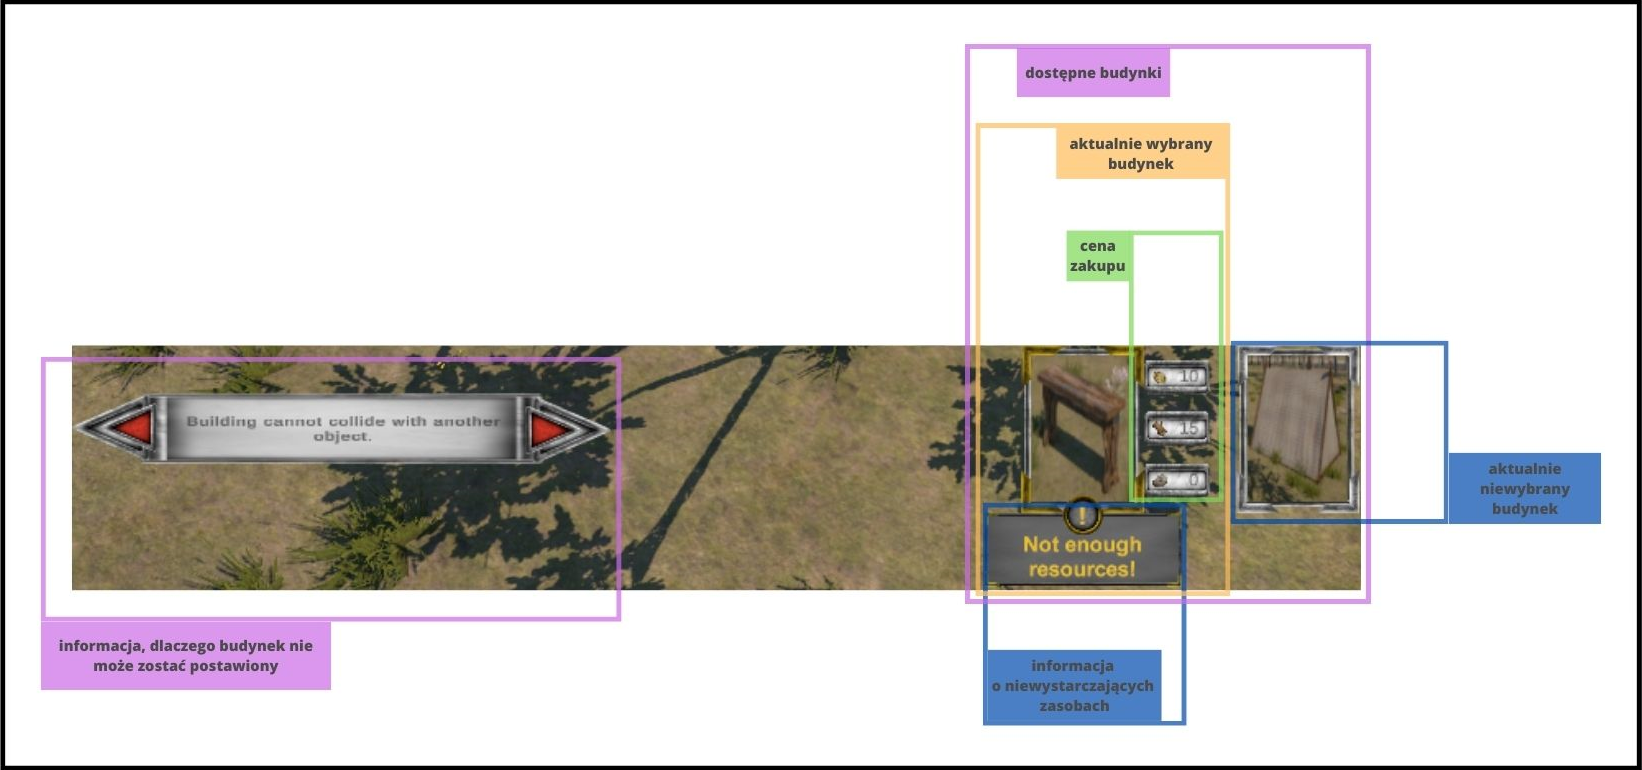
\includegraphics[width=0.9\textwidth]{images/ui/opis_ekementow_budowanie.png}
    \caption{Implementacja menu stawiania budynków, na którym pokazane są możliwe do zbudowania budowle 
    i szczegółowe informacje o ich dostępności.
    }\label{fig:compass}
\end{figure}

\subsection{Menu wydawania komend}

\begin{figure}[htbp]
    \centering
    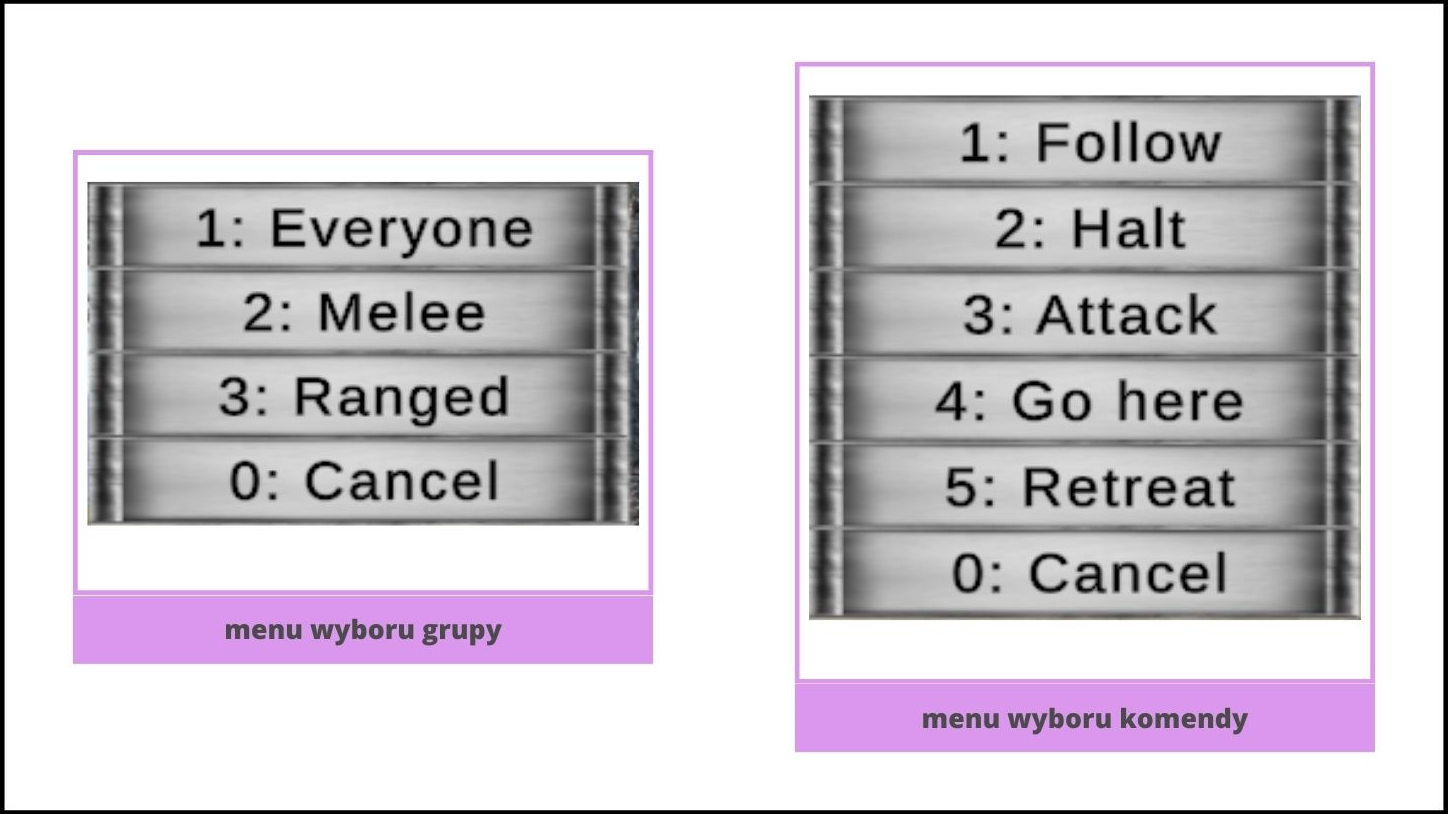
\includegraphics[width=0.9\textwidth]{images/ui/opis_ekementow_mwnu_wyboru_komendy.png}
    \caption{Implementacja menu wydawania komend}\label{fig:c}
\end{figure}
\subsection{Menu zapisu}

\subsection{Notatnik z zadaniami}

\subsection{Informacja o możliwej czynności}

\subsection{Menu końca gry}